\chapter{Examining MongoDB Query Features}
%Intro\footnotemark\\
\par Lorem ipsum dolor sit amet, consectetur adipiscing elit. Aliquam facilisis massa quis orci volutpat, ut dictum tellus pulvinar. Nam vulputate diam a leo dignissim varius. Aenean nec tellus malesuada, tristique libero vitae, lacinia nibh. Donec quam libero, accumsan sollicitudin massa a, dictum gravida mauris.
\begin{spacing}{1.2}
%note en bas de page
\section{Restoring a .bson file }
\par Lorem ipsum dolor sit amet, consectetur adipiscing elit. Aliquam facilisis massa quis orci volutpat, ut dictum tellus pulvinar. Nam vulputate diam a leo dignissim varius. Aenean nec tellus malesuada, tristique libero vitae, lacinia nibh. Donec quam libero, accumsan sollicitudin massa a, dictum gravida mauris
\\
\begin{figure}[!htb] 
\begin{center} 
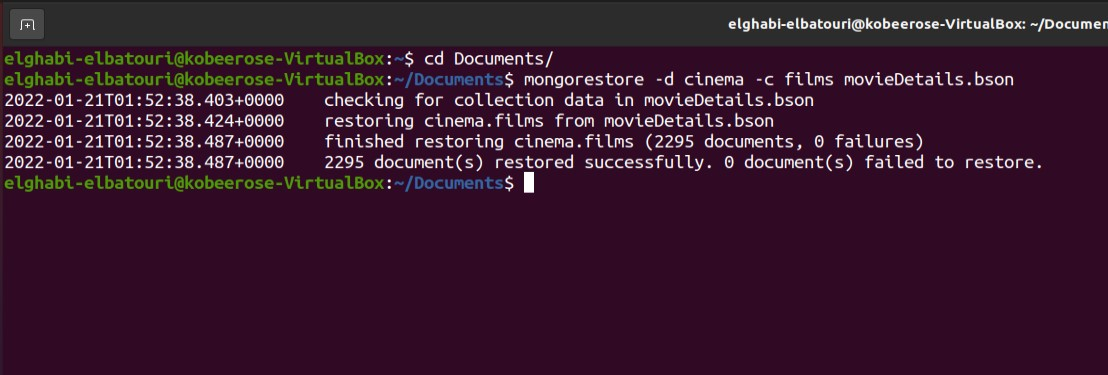
\includegraphics[width=1\linewidth]{Pictures/MongoDB/Examining MongoDB Query Features/Restoring a .bson file/Restore movieDetails in the DB} 
\end{center} 
\caption{Restore movieDetails in the DB} 
\end{figure}  \FloatBarrier
\\

\par Lorem ipsum dolor sit amet, consectetur adipiscing elit. Aliquam facilisis massa quis orci volutpat, ut dictum tellus pulvinar. Nam vulputate diam a leo dignissim varius. Aenean nec tellus malesuada, tristique libero vitae, lacinia nibh. Donec quam libero, accumsan sollicitudin massa a, dictum gravida mauris
\\
\begin{figure}[!htb] 
\begin{center} 
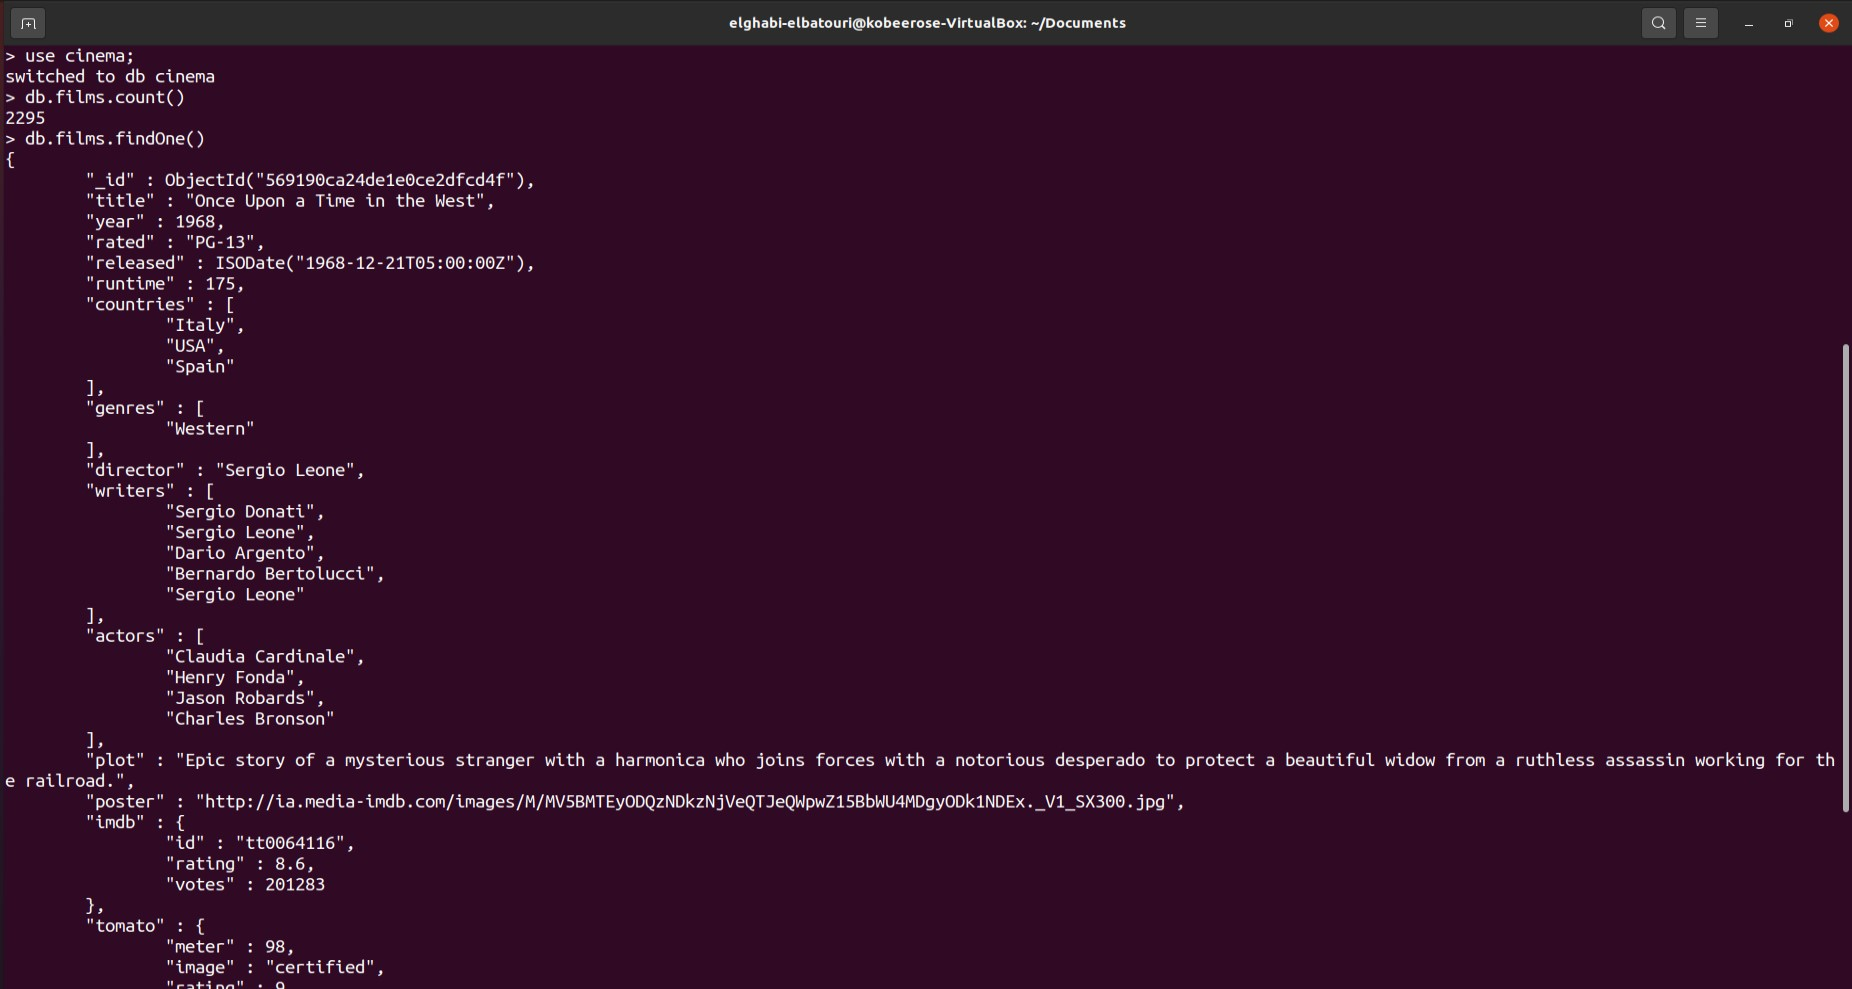
\includegraphics[width=1\linewidth]{Pictures/MongoDB/Examining MongoDB Query Features/Restoring a .bson file/Checking the data in mongo shell} 
\end{center} 
\caption{Checking the data in mongo shell} 
\end{figure}  \FloatBarrier
\\
\section{Index management }
\par Lorem ipsum dolor sit amet, consectetur adipiscing elit. Aliquam facilisis massa quis orci volutpat, ut dictum tellus pulvinar. Nam vulputate diam a leo dignissim varius. Aenean nec tellus malesuada, tristique libero vitae, lacinia nibh. Donec quam libero, accumsan sollicitudin massa a, dictum gravida mauris
\\
\begin{figure}[!htb] 
\begin{center} 
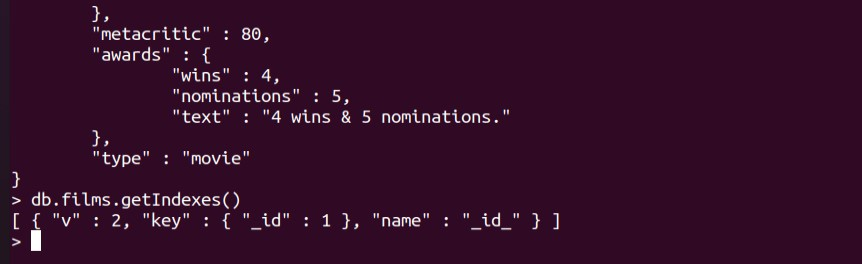
\includegraphics[width=1\linewidth]{Pictures/MongoDB/Examining MongoDB Query Features/Index management/Displaying indexes} 
\end{center} 
\caption{Displaying indexes} 
\end{figure}  \FloatBarrier
\\

\par Lorem ipsum dolor sit amet, consectetur adipiscing elit. Aliquam facilisis massa quis orci volutpat, ut dictum tellus pulvinar. Nam vulputate diam a leo dignissim varius. Aenean nec tellus malesuada, tristique libero vitae, lacinia nibh. Donec quam libero, accumsan sollicitudin massa a, dictum gravida mauris
\\
\begin{figure}[!htb] 
\begin{center} 
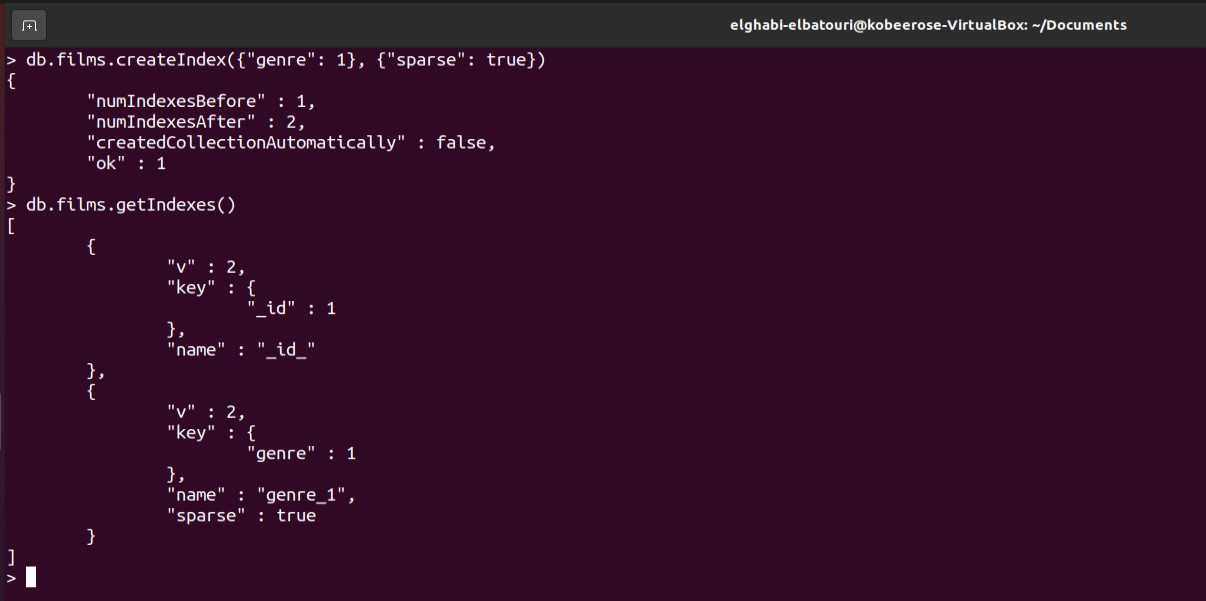
\includegraphics[width=1\linewidth]{Pictures/MongoDB/Examining MongoDB Query Features/Index management/Creating an Index} 
\end{center} 
\caption{Creating an Index} 
\end{figure}  \FloatBarrier
\\

\par Lorem ipsum dolor sit amet, consectetur adipiscing elit. Aliquam facilisis massa quis orci volutpat, ut dictum tellus pulvinar. Nam vulputate diam a leo dignissim varius. Aenean nec tellus malesuada, tristique libero vitae, lacinia nibh. Donec quam libero, accumsan sollicitudin massa a, dictum gravida mauris
\\
\begin{figure}[!htb] 
\begin{center} 
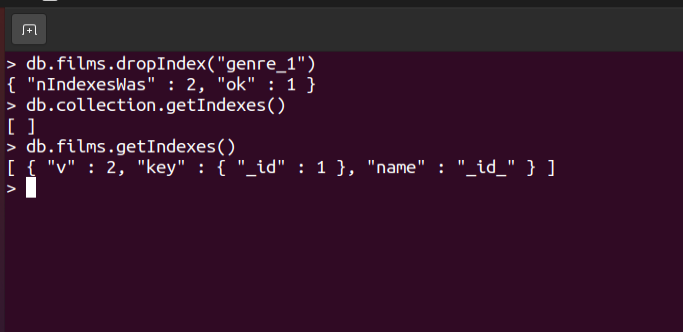
\includegraphics[width=1\linewidth]{Pictures/MongoDB/Examining MongoDB Query Features/Index management/Dropping an index} 
\end{center} 
\caption{Dropping an index} 
\end{figure}  \FloatBarrier
\\

\par Lorem ipsum dolor sit amet, consectetur adipiscing elit. Aliquam facilisis massa quis orci volutpat, ut dictum tellus pulvinar. Nam vulputate diam a leo dignissim varius. Aenean nec tellus malesuada, tristique libero vitae, lacinia nibh. Donec quam libero, accumsan sollicitudin massa a, dictum gravida mauris
\\
\begin{figure}[!htb] 
\begin{center} 
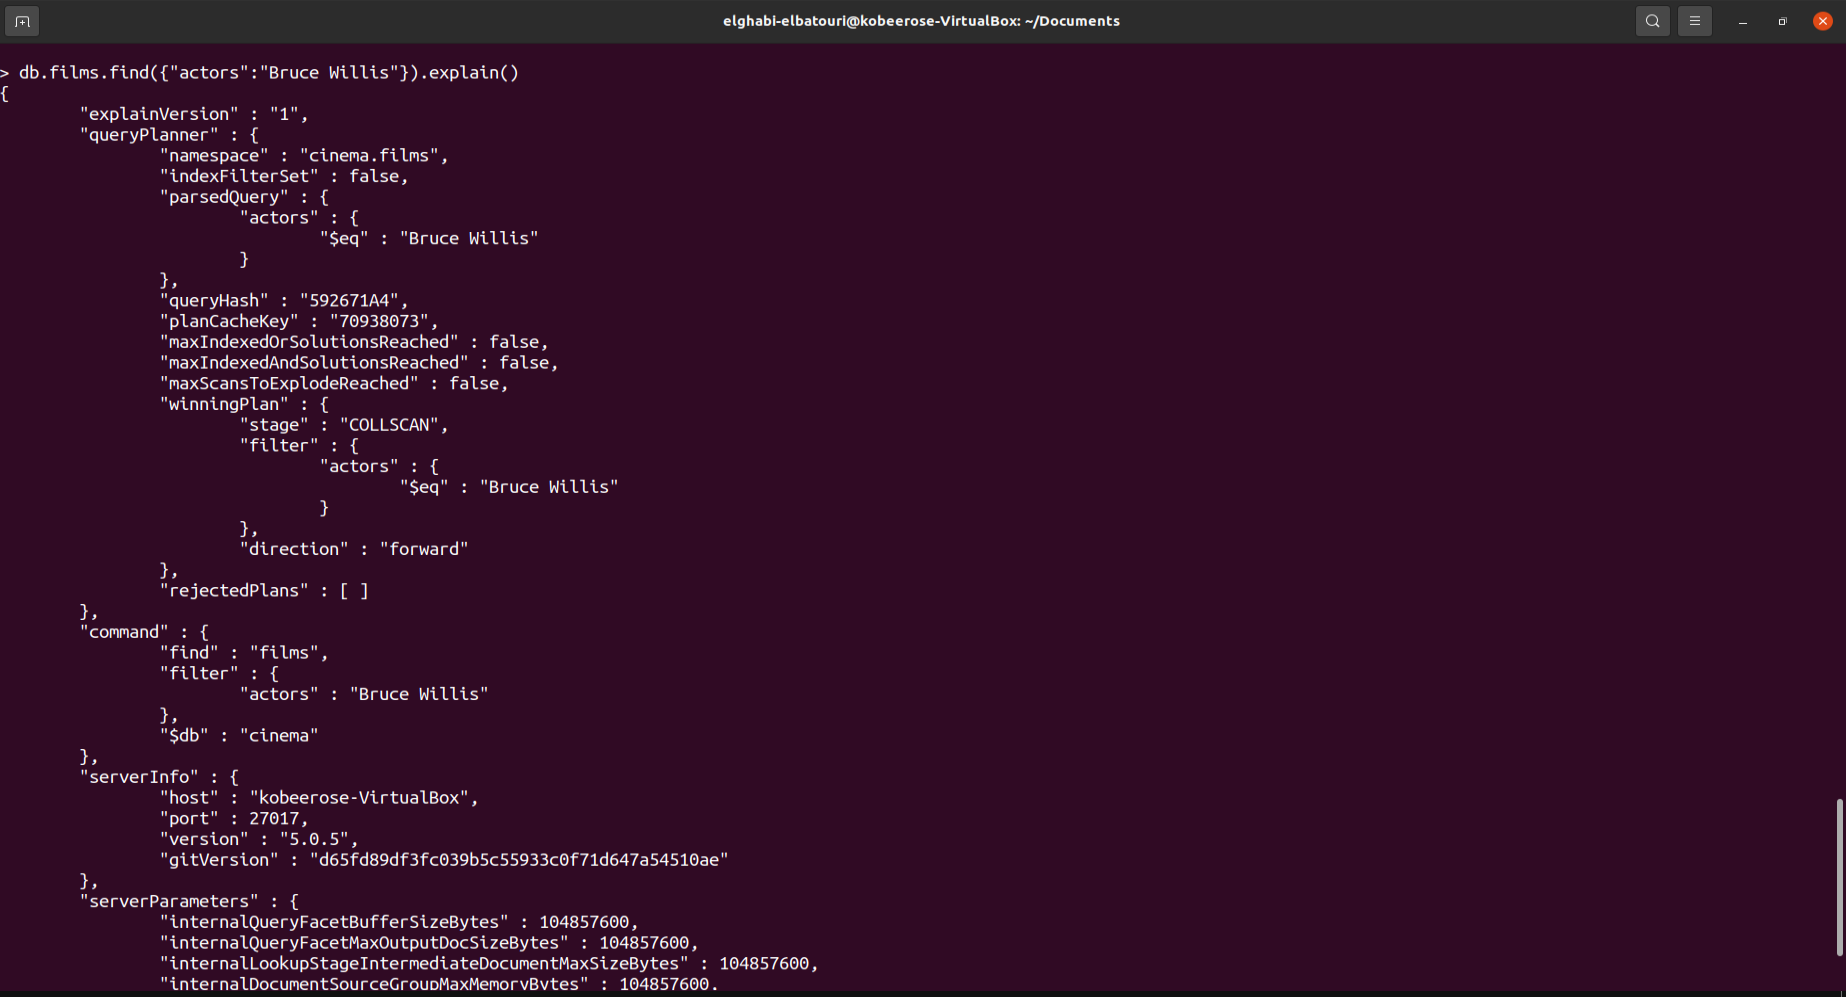
\includegraphics[width=1\linewidth]{Pictures/MongoDB/Examining MongoDB Query Features/Index management/explain() command} 
\end{center} 
\caption{explain() command} 
\end{figure}  \FloatBarrier
\\

\section{Document search }
\par Lorem ipsum dolor sit amet, consectetur adipiscing elit. Aliquam facilisis massa quis orci volutpat, ut dictum tellus pulvinar. Nam vulputate diam a leo dignissim varius. Aenean nec tellus malesuada, tristique libero vitae, lacinia nibh. Donec quam libero, accumsan sollicitudin massa a, dictum gravida mauris
\\
\begin{figure}[!htb] 
\begin{center} 
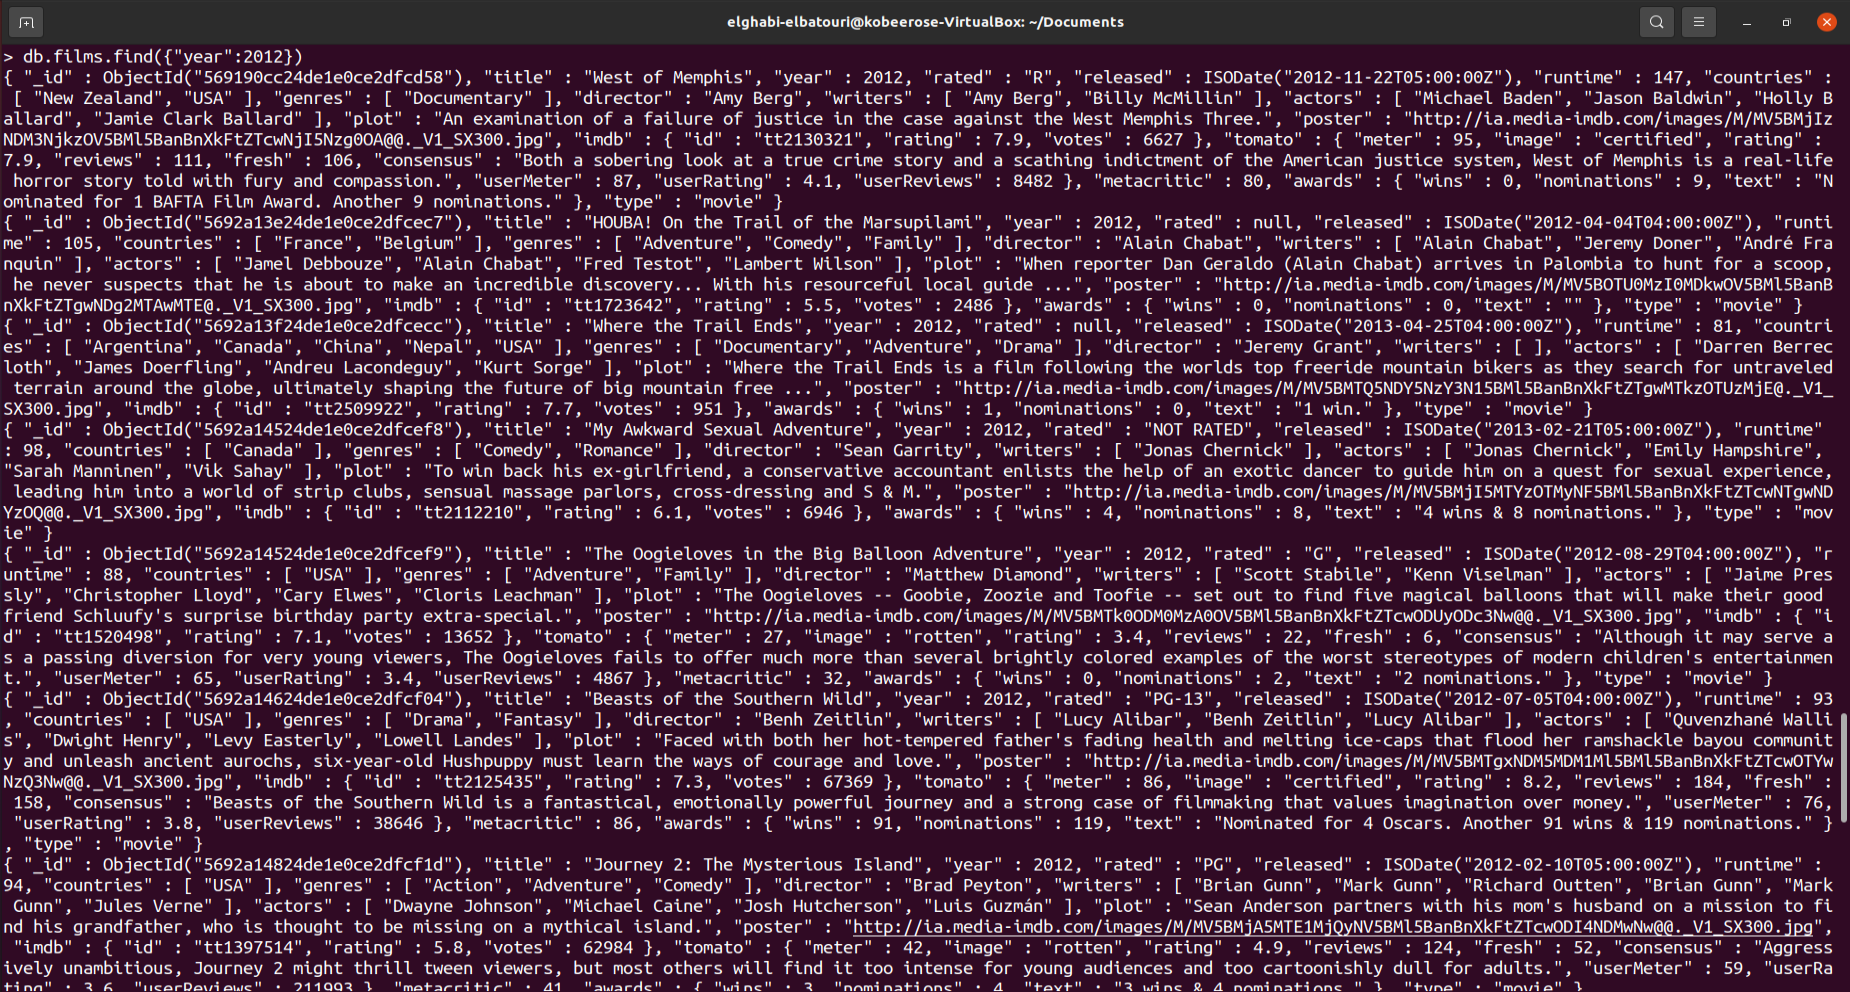
\includegraphics[width=1\linewidth]{Pictures/MongoDB/Examining MongoDB Query Features/Document search/Searching for 2012 films} 
\end{center} 
\caption{Searching for 2012 films} 
\end{figure}  \FloatBarrier
\\

\par Lorem ipsum dolor sit amet, consectetur adipiscing elit. Aliquam facilisis massa quis orci volutpat, ut dictum tellus pulvinar. Nam vulputate diam a leo dignissim varius. Aenean nec tellus malesuada, tristique libero vitae, lacinia nibh. Donec quam libero, accumsan sollicitudin massa a, dictum gravida mauris
\\
\begin{figure}[!htb] 
\begin{center} 
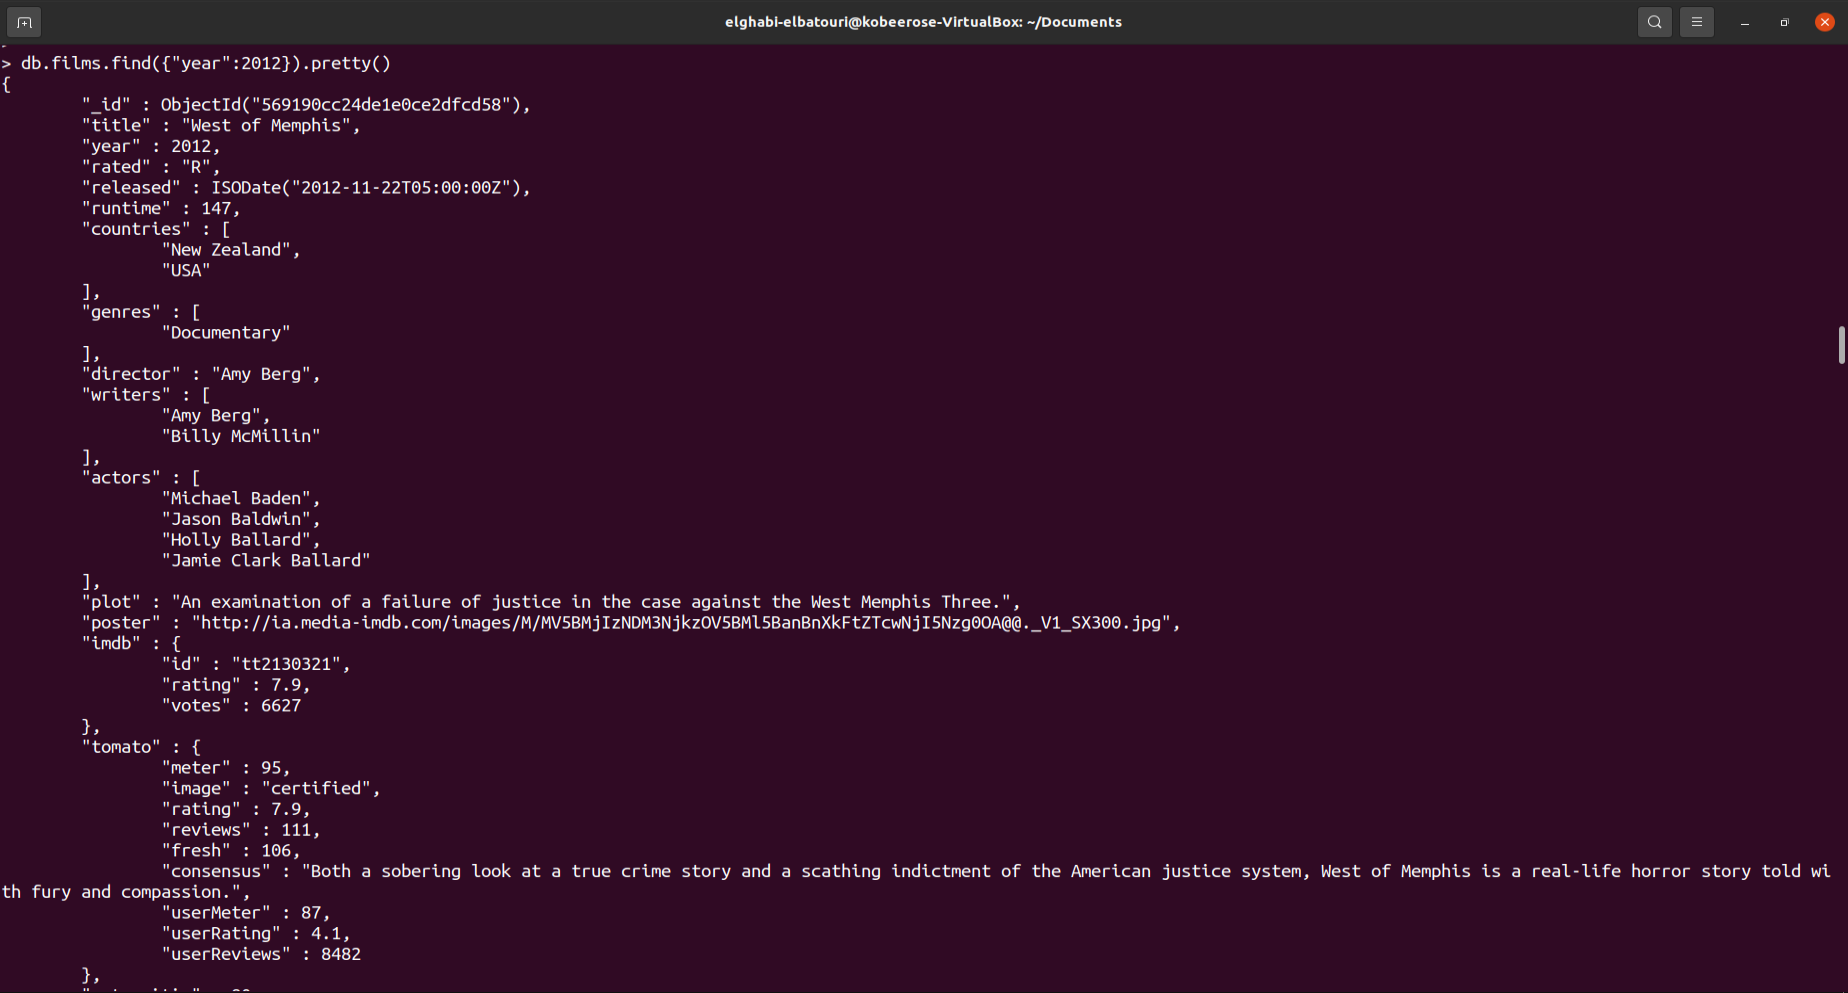
\includegraphics[width=1\linewidth]{Pictures/MongoDB/Examining MongoDB Query Features/Document search/Formatting the search results} 
\end{center} 
\caption{Formatting the search results} 
\end{figure}  \FloatBarrier
\\

\par Lorem ipsum dolor sit amet, consectetur adipiscing elit. Aliquam facilisis massa quis orci volutpat, ut dictum tellus pulvinar. Nam vulputate diam a leo dignissim varius. Aenean nec tellus malesuada, tristique libero vitae, lacinia nibh. Donec quam libero, accumsan sollicitudin massa a, dictum gravida mauris
\\
\begin{figure}[!htb] 
\begin{center} 
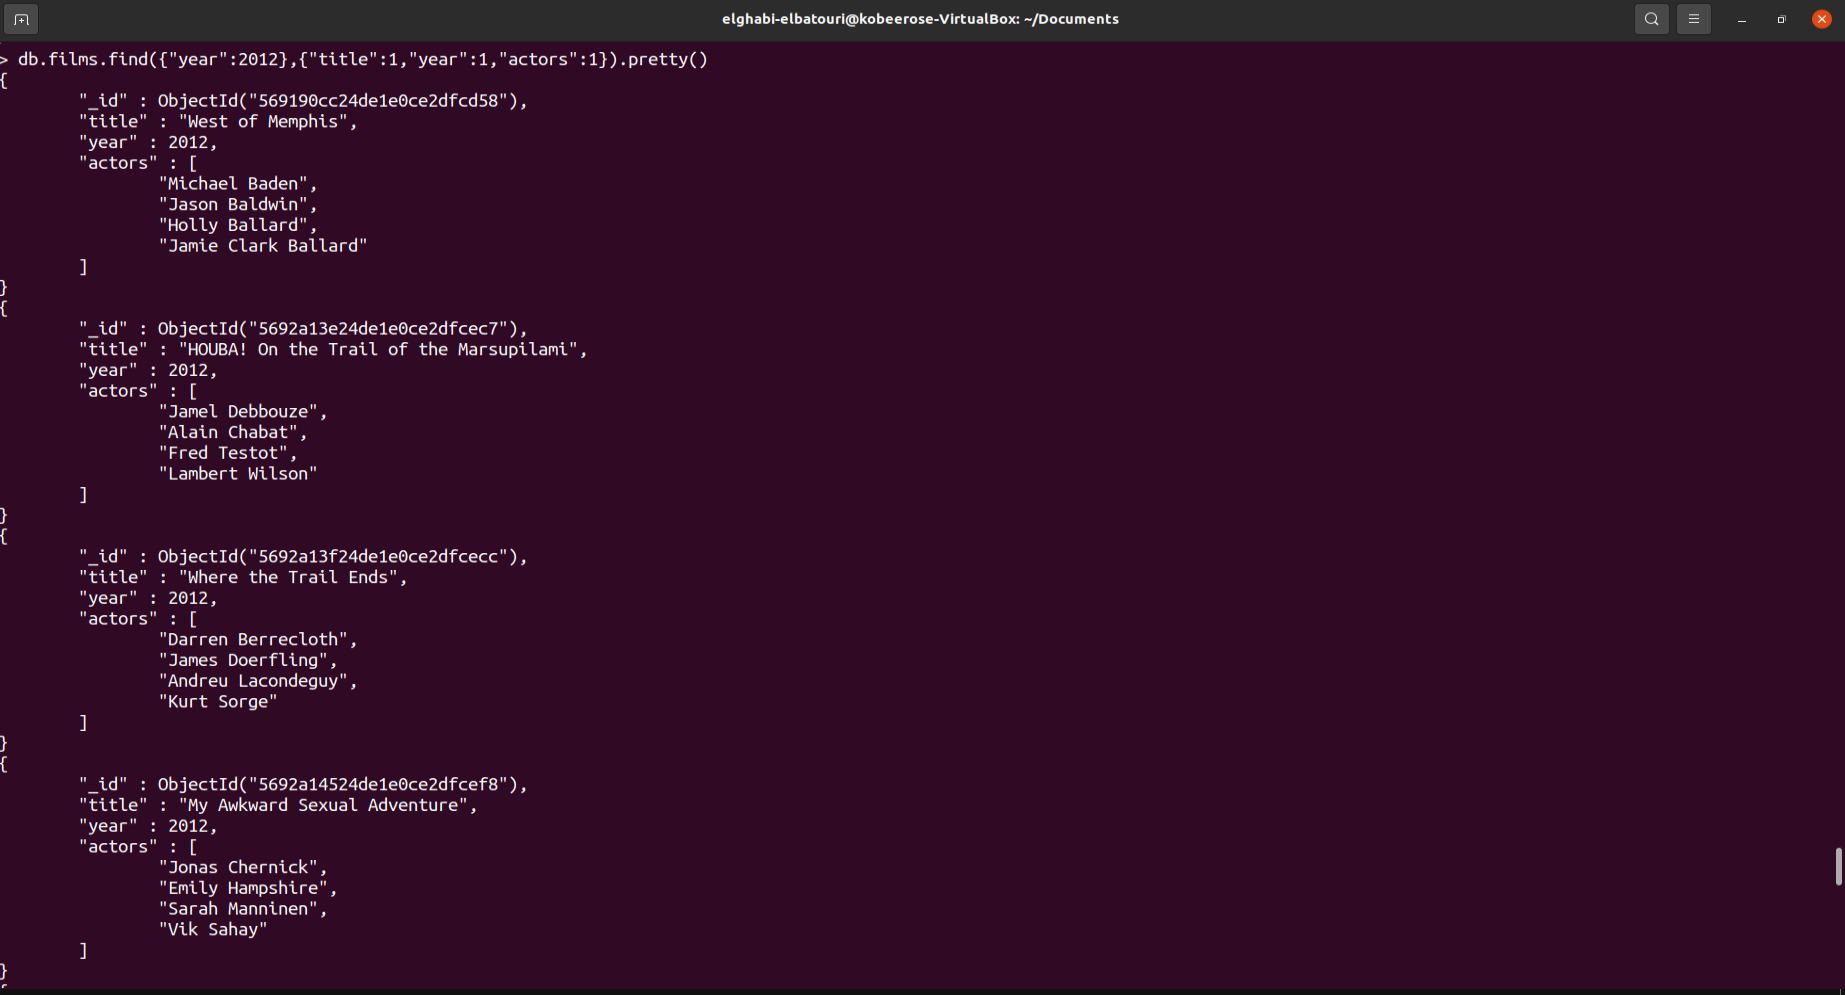
\includegraphics[width=1\linewidth]{Pictures/MongoDB/Examining MongoDB Query Features/Document search/Projection} 
\end{center} 
\caption{Projection} 
\end{figure}  \FloatBarrier
\\

\par Lorem ipsum dolor sit amet, consectetur adipiscing elit. Aliquam facilisis massa quis orci volutpat, ut dictum tellus pulvinar. Nam vulputate diam a leo dignissim varius. Aenean nec tellus malesuada, tristique libero vitae, lacinia nibh. Donec quam libero, accumsan sollicitudin massa a, dictum gravida mauris
\\
\begin{figure}[!htb] 
\begin{center} 
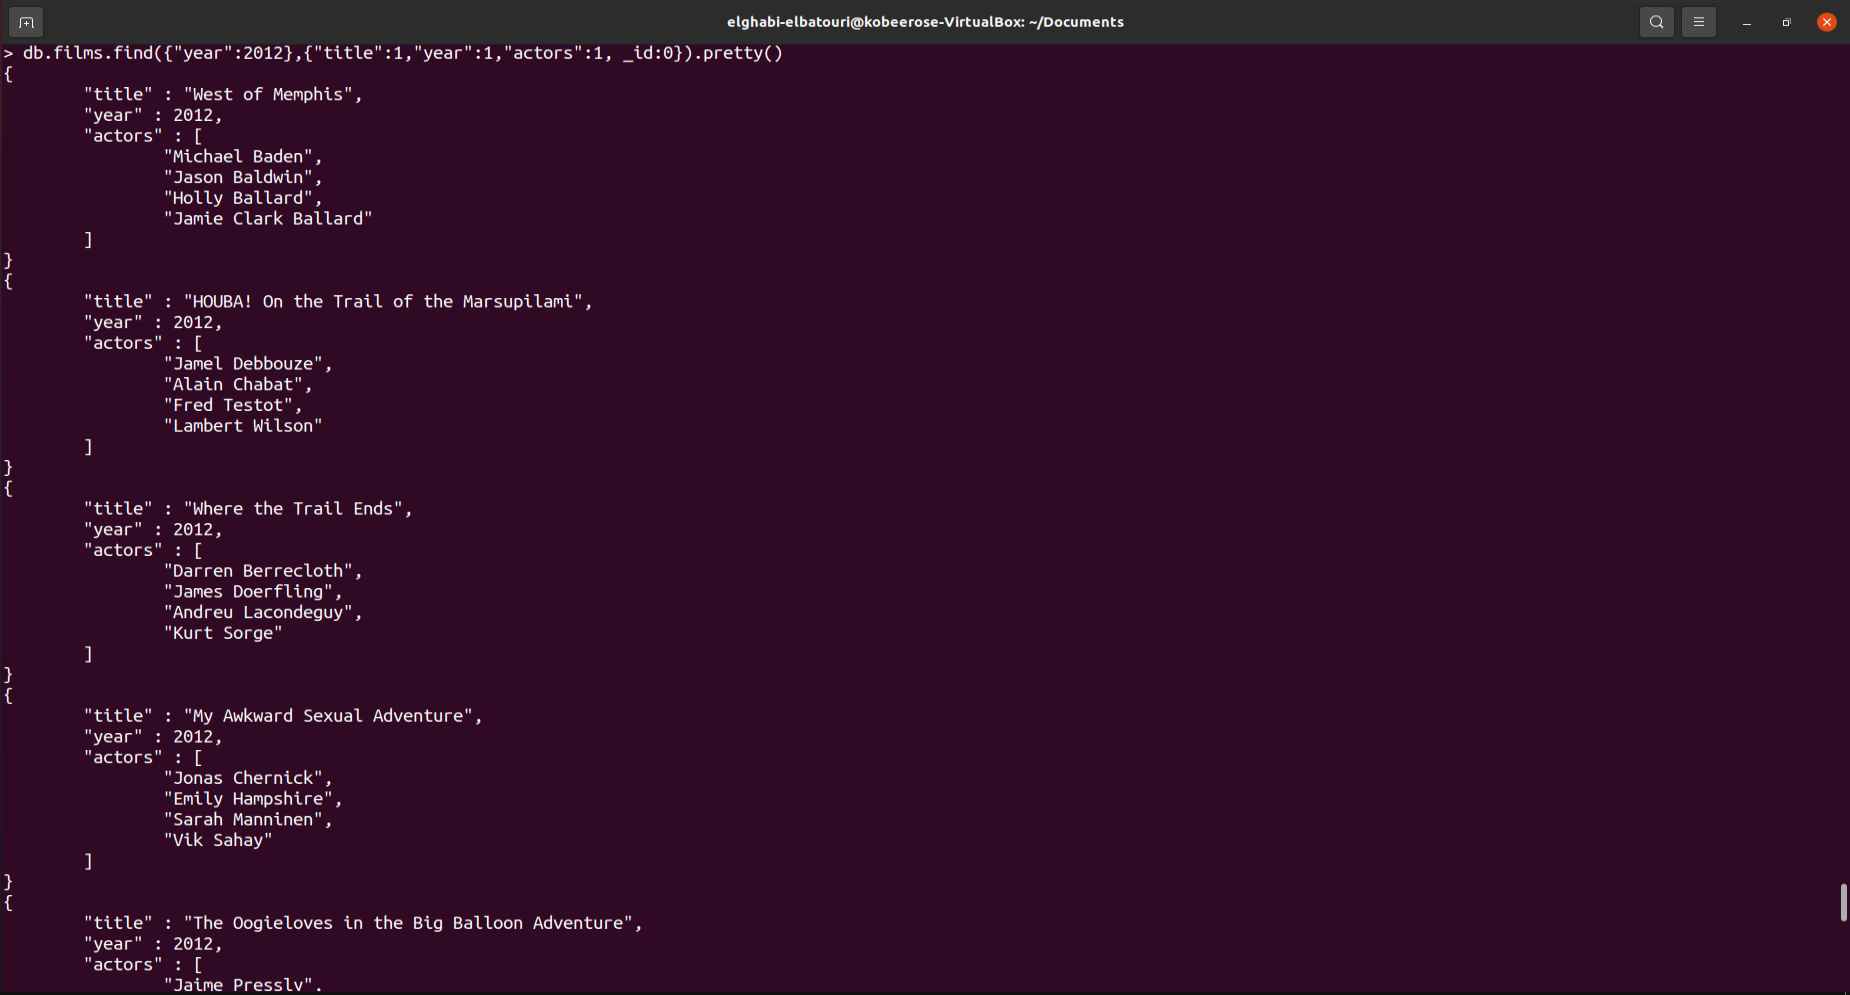
\includegraphics[width=1\linewidth]{Pictures/MongoDB/Examining MongoDB Query Features/Document search/Including and excluding fields} 
\end{center} 
\caption{Including and excluding fields} 
\end{figure}  \FloatBarrier
\\

\par Lorem ipsum dolor sit amet, consectetur adipiscing elit. Aliquam facilisis massa quis orci volutpat, ut dictum tellus pulvinar. Nam vulputate diam a leo dignissim varius. Aenean nec tellus malesuada, tristique libero vitae, lacinia nibh. Donec quam libero, accumsan sollicitudin massa a, dictum gravida mauris
\\
\begin{figure}[!htb] 
\begin{center} 
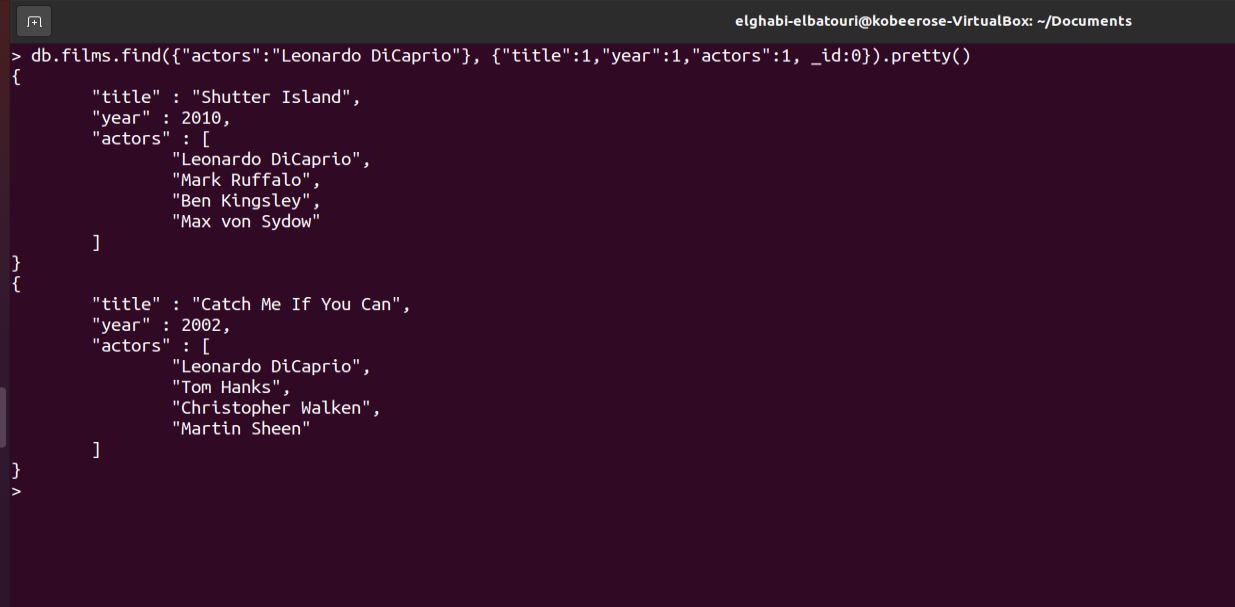
\includegraphics[width=1\linewidth]{Pictures/MongoDB/Examining MongoDB Query Features/Document search/Searching in tables} 
\end{center} 
\caption{Searching in tables} 
\end{figure}  \FloatBarrier
\\

\par Lorem ipsum dolor sit amet, consectetur adipiscing elit. Aliquam facilisis massa quis orci volutpat, ut dictum tellus pulvinar. Nam vulputate diam a leo dignissim varius. Aenean nec tellus malesuada, tristique libero vitae, lacinia nibh. Donec quam libero, accumsan sollicitudin massa a, dictum gravida mauris
\\
\begin{figure}[!htb] 
\begin{center} 
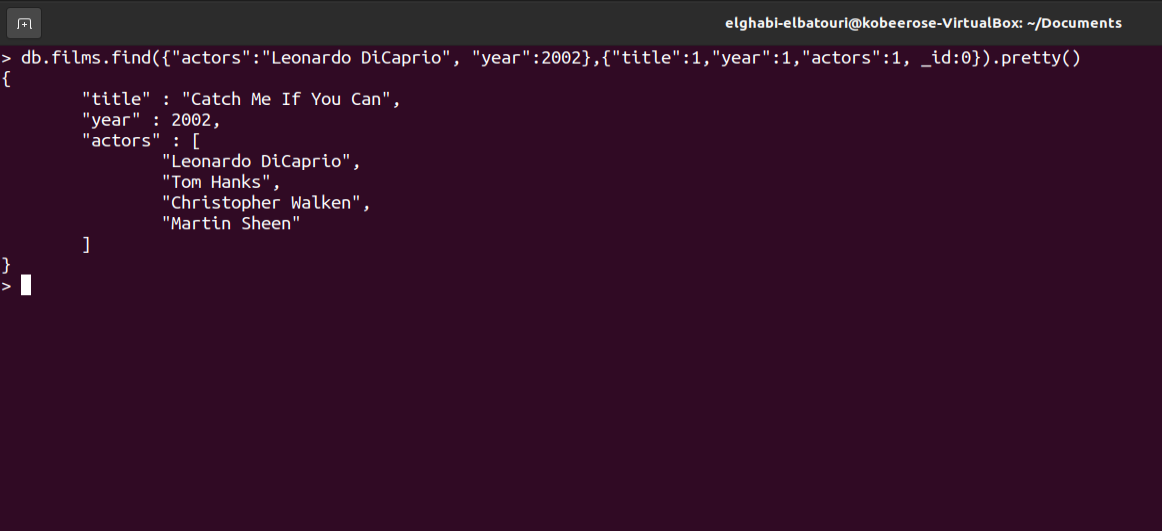
\includegraphics[width=1\linewidth]{Pictures/MongoDB/Examining MongoDB Query Features/Document search/Combining multiple filters} 
\end{center} 
\caption{Combining multiple filters} 
\end{figure}  \FloatBarrier
\\

\par Lorem ipsum dolor sit amet, consectetur adipiscing elit. Aliquam facilisis massa quis orci volutpat, ut dictum tellus pulvinar. Nam vulputate diam a leo dignissim varius. Aenean nec tellus malesuada, tristique libero vitae, lacinia nibh. Donec quam libero, accumsan sollicitudin massa a, dictum gravida mauris
\\
\begin{figure}[!htb] 
\begin{center} 
\includegraphics[width=1\linewidth]{Pictures/MongoDB/Examining MongoDB Query Features/Document search/Using \$in operator} 
\end{center} 
\caption{Using \$in operator} 
\end{figure}  \FloatBarrier
\\

\par Lorem ipsum dolor sit amet, consectetur adipiscing elit. Aliquam facilisis massa quis orci volutpat, ut dictum tellus pulvinar. Nam vulputate diam a leo dignissim varius. Aenean nec tellus malesuada, tristique libero vitae, lacinia nibh. Donec quam libero, accumsan sollicitudin massa a, dictum gravida mauris
\\
\begin{figure}[!htb] 
\begin{center} 
\includegraphics[width=1\linewidth]{Pictures/MongoDB/Examining MongoDB Query Features/Document search/Using \$all operator} 
\end{center} 
\caption{Using \$all operator} 
\end{figure}  \FloatBarrier
\\

\section{Advanced search }
\par Lorem ipsum dolor sit amet, consectetur adipiscing elit. Aliquam facilisis massa quis orci volutpat, ut dictum tellus pulvinar. Nam vulputate diam a leo dignissim varius. Aenean nec tellus malesuada, tristique libero vitae, lacinia nibh. Donec quam libero, accumsan sollicitudin massa a, dictum gravida mauris
\\
\begin{figure}[!htb] 
\begin{center} 
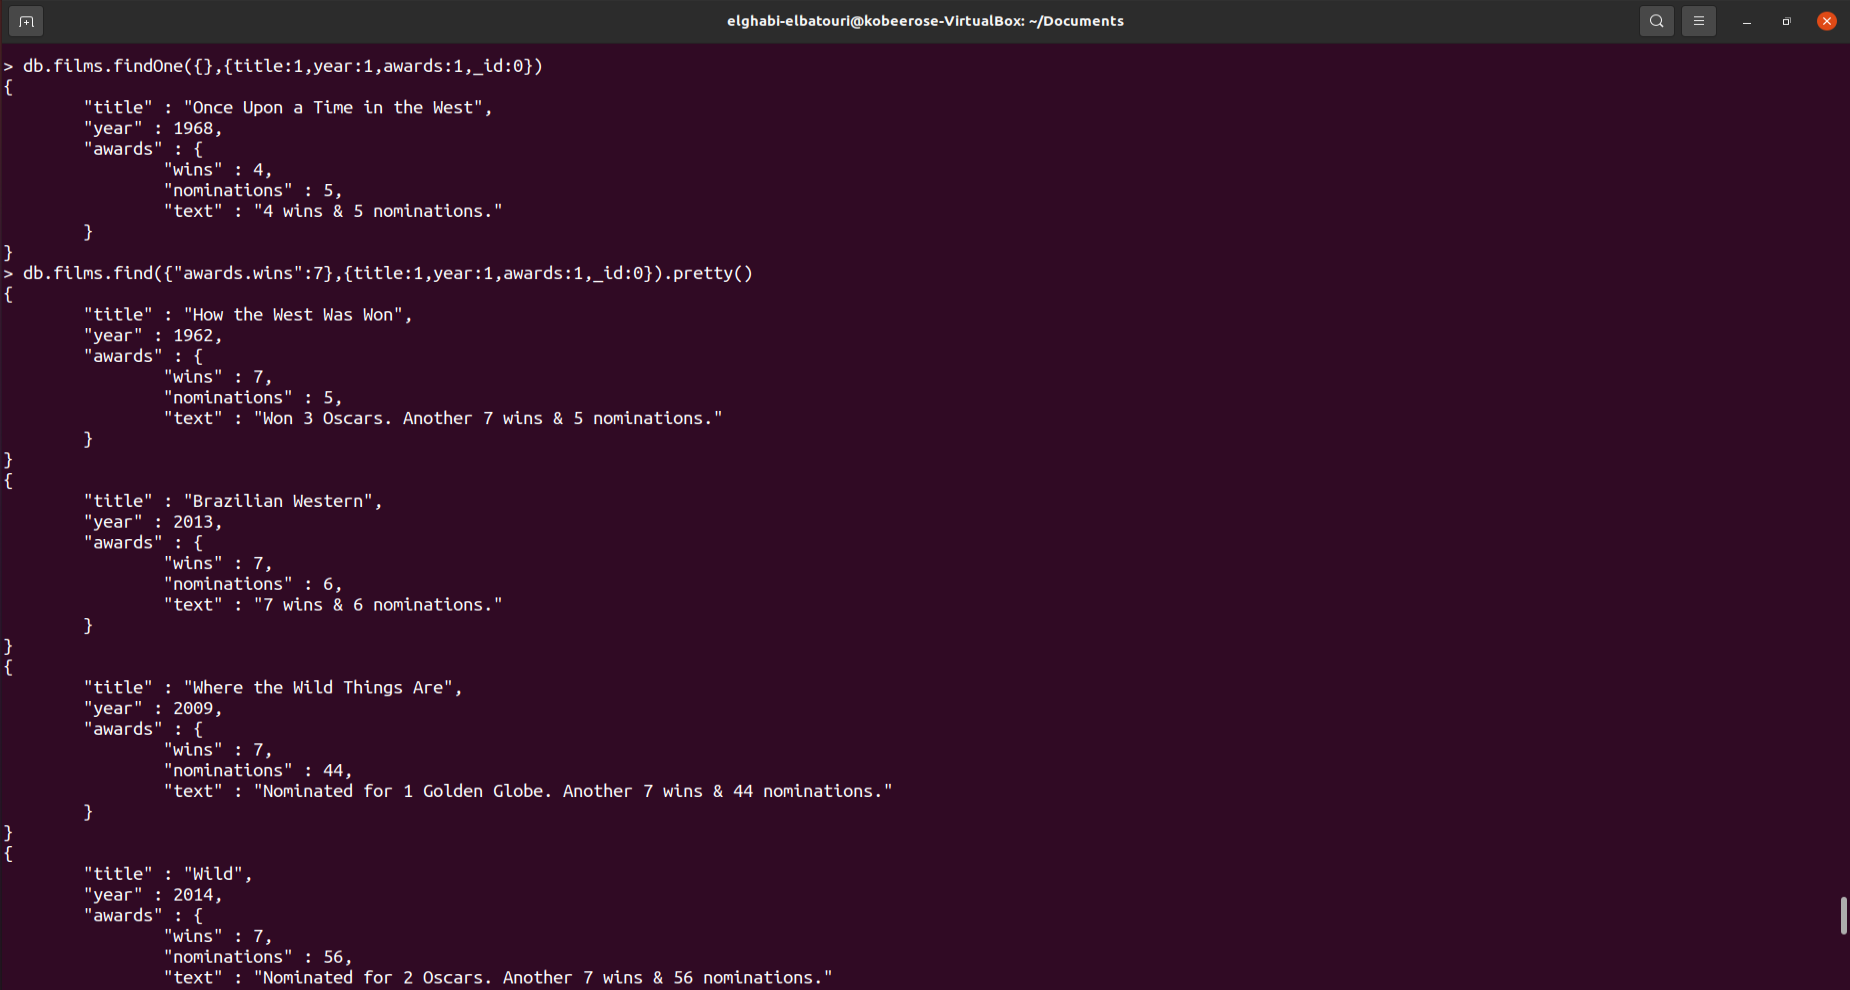
\includegraphics[width=1\linewidth]{Pictures/MongoDB/Examining MongoDB Query Features/Advanced search/Checking nested documents} 
\end{center} 
\caption{Checking nested documents} 
\end{figure}  \FloatBarrier
\\

\par Lorem ipsum dolor sit amet, consectetur adipiscing elit. Aliquam facilisis massa quis orci volutpat, ut dictum tellus pulvinar. Nam vulputate diam a leo dignissim varius. Aenean nec tellus malesuada, tristique libero vitae, lacinia nibh. Donec quam libero, accumsan sollicitudin massa a, dictum gravida mauris
\\
\begin{figure}[!htb] 
\begin{center} 
\includegraphics[width=1\linewidth]{Pictures/MongoDB/Examining MongoDB Query Features/Advanced search/Using \$ne operator} 
\end{center} 
\caption{Using \$ne operator} 
\end{figure}  \FloatBarrier
\\

\par Lorem ipsum dolor sit amet, consectetur adipiscing elit. Aliquam facilisis massa quis orci volutpat, ut dictum tellus pulvinar. Nam vulputate diam a leo dignissim varius. Aenean nec tellus malesuada, tristique libero vitae, lacinia nibh. Donec quam libero, accumsan sollicitudin massa a, dictum gravida mauris
\\
\begin{figure}[!htb] 
\begin{center} 
\includegraphics[width=1\linewidth]{Pictures/MongoDB/Examining MongoDB Query Features/Advanced search/Using \$gte operator} 
\end{center} 
\caption{Using \$gte operator} 
\end{figure}  \FloatBarrier
\\

\par Lorem ipsum dolor sit amet, consectetur adipiscing elit. Aliquam facilisis massa quis orci volutpat, ut dictum tellus pulvinar. Nam vulputate diam a leo dignissim varius. Aenean nec tellus malesuada, tristique libero vitae, lacinia nibh. Donec quam libero, accumsan sollicitudin massa a, dictum gravida mauris
\\
\begin{figure}[!htb] 
\begin{center} 
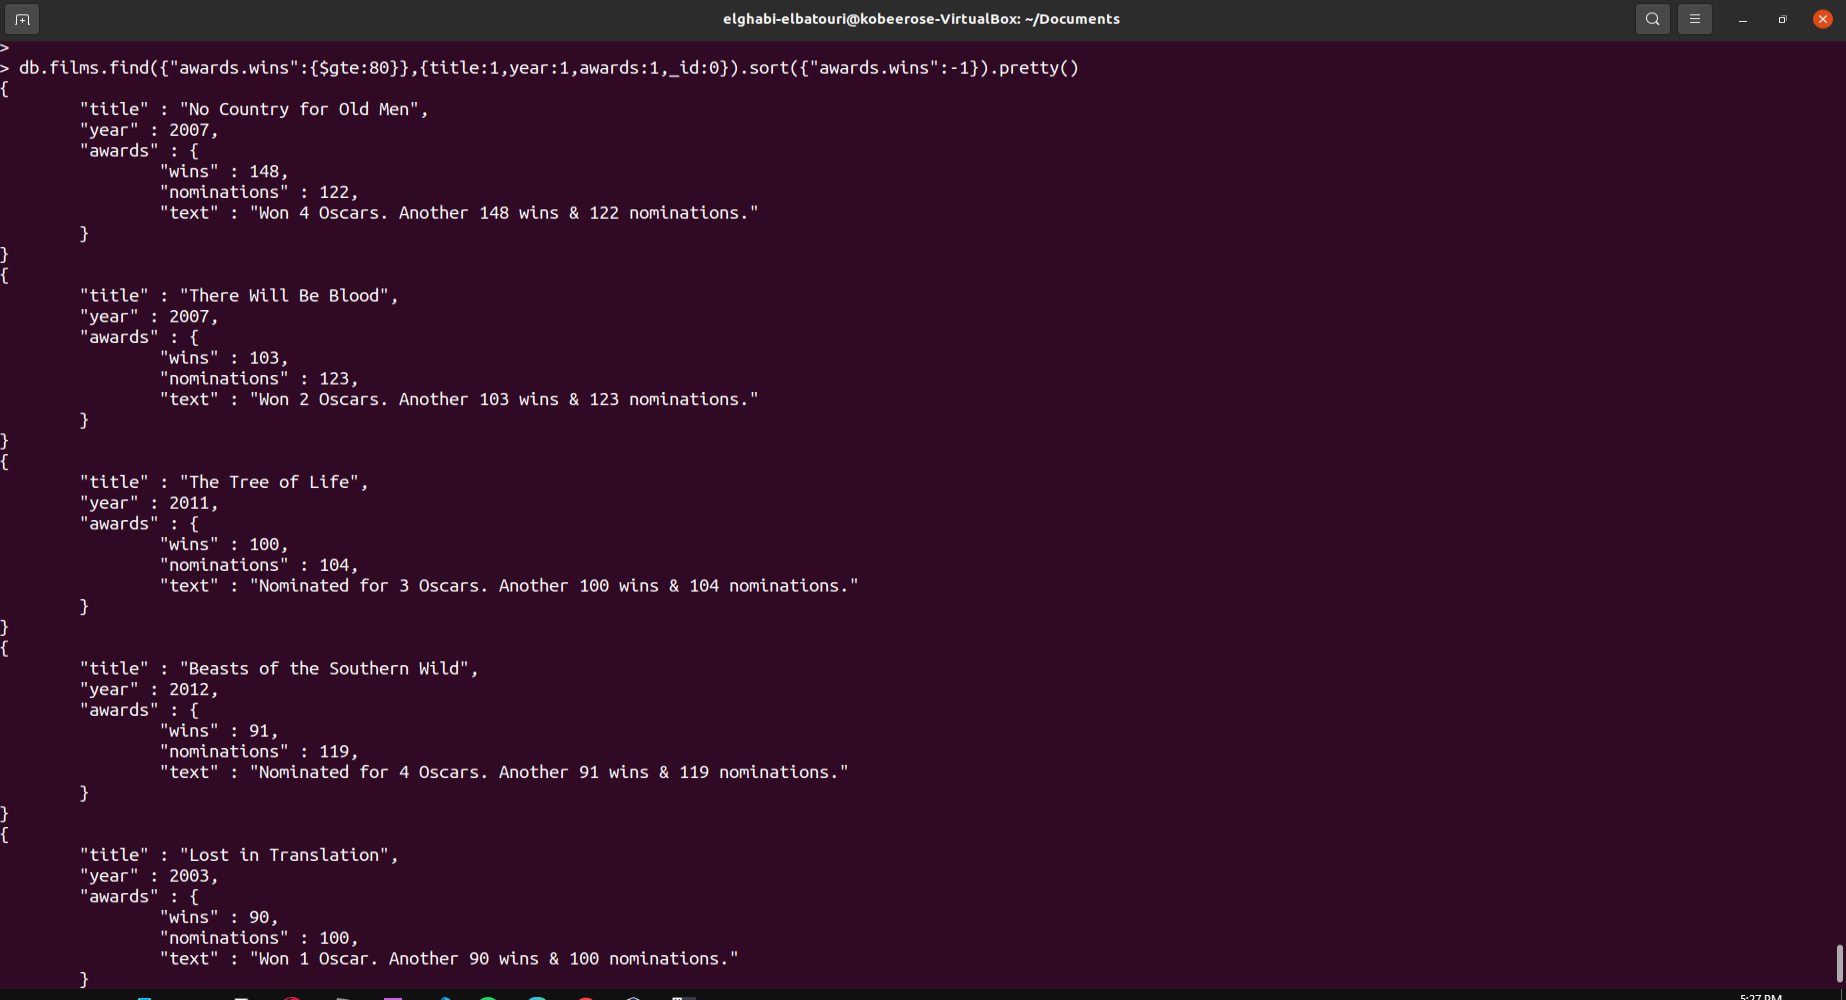
\includegraphics[width=1\linewidth]{Pictures/MongoDB/Examining MongoDB Query Features/Advanced search/Sorting results} 
\end{center} 
\caption{Sorting results} 
\end{figure}  \FloatBarrier
\\
\section{Inserting documents }
\par Lorem ipsum dolor sit amet, consectetur adipiscing elit. Aliquam facilisis massa quis orci volutpat, ut dictum tellus pulvinar. Nam vulputate diam a leo dignissim varius. Aenean nec tellus malesuada, tristique libero vitae, lacinia nibh. Donec quam libero, accumsan sollicitudin massa a, dictum gravida mauris
\\
\begin{figure}[!htb] 
\begin{center} 
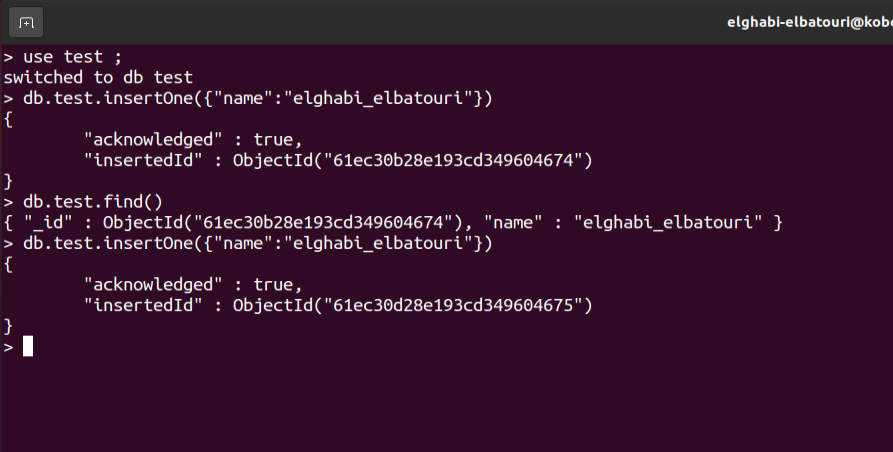
\includegraphics[width=1\linewidth]{Pictures/MongoDB/Examining MongoDB Query Features/Inserting documents/Inserting object and checking} 
\end{center} 
\caption{Inserting object and checking} 
\end{figure}  \FloatBarrier
\\

\par Lorem ipsum dolor sit amet, consectetur adipiscing elit. Aliquam facilisis massa quis orci volutpat, ut dictum tellus pulvinar. Nam vulputate diam a leo dignissim varius. Aenean nec tellus malesuada, tristique libero vitae, lacinia nibh. Donec quam libero, accumsan sollicitudin massa a, dictum gravida mauris
\\
\begin{figure}[!htb] 
\begin{center} 
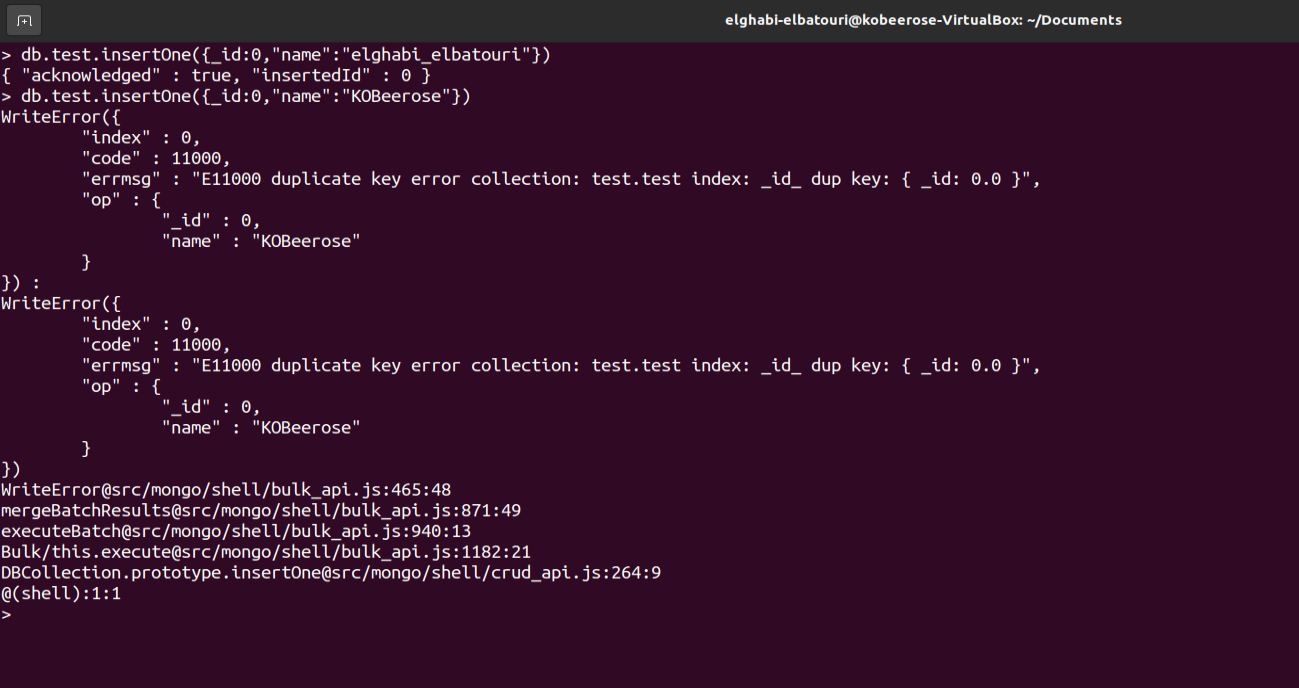
\includegraphics[width=1\linewidth]{Pictures/MongoDB/Examining MongoDB Query Features/Inserting documents/Error of inserting in the same id} 
\end{center} 
\caption{Error of inserting in the same id} 
\end{figure}  \FloatBarrier
\\

\par Lorem ipsum dolor sit amet, consectetur adipiscing elit. Aliquam facilisis massa quis orci volutpat, ut dictum tellus pulvinar. Nam vulputate diam a leo dignissim varius. Aenean nec tellus malesuada, tristique libero vitae, lacinia nibh. Donec quam libero, accumsan sollicitudin massa a, dictum gravida mauris
\\
\begin{figure}[!htb] 
\begin{center} 
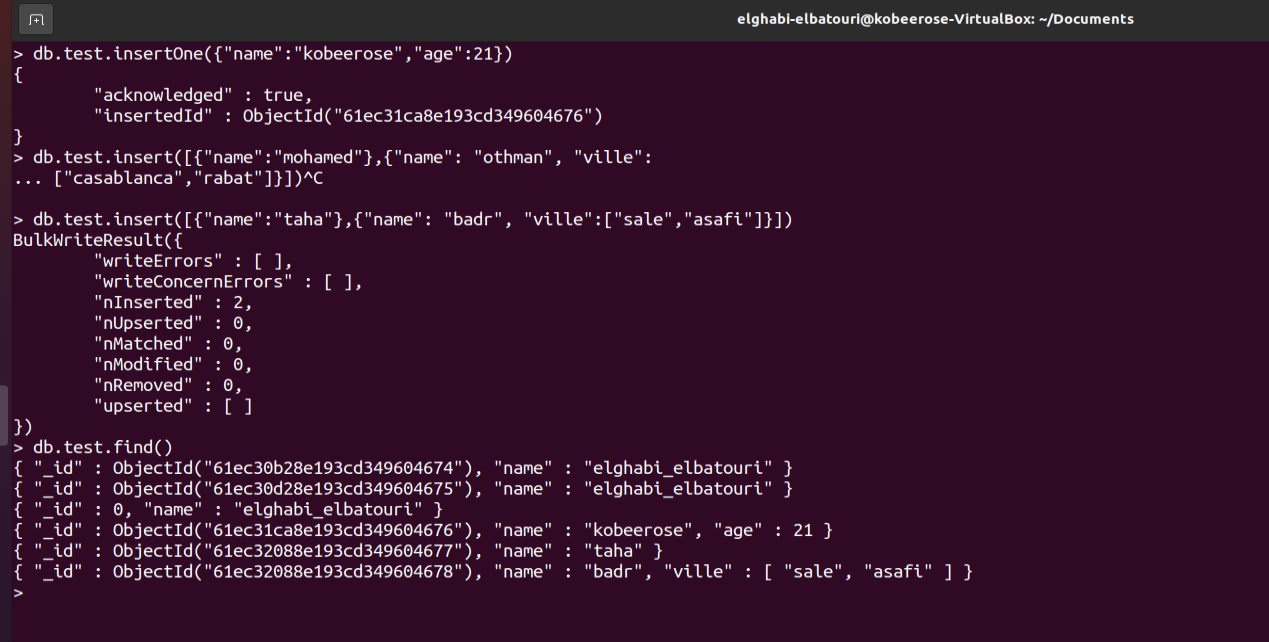
\includegraphics[width=1\linewidth]{Pictures/MongoDB/Examining MongoDB Query Features/Inserting documents/Documents with different structure in same collection} 
\end{center} 
\caption{Documents with different structure in same collection} 
\end{figure}  \FloatBarrier
\\
\section{Deleting and Updating documents }
\par Lorem ipsum dolor sit amet, consectetur adipiscing elit. Aliquam facilisis massa quis orci volutpat, ut dictum tellus pulvinar. Nam vulputate diam a leo dignissim varius. Aenean nec tellus malesuada, tristique libero vitae, lacinia nibh. Donec quam libero, accumsan sollicitudin massa a, dictum gravida mauris
\\
\begin{figure}[!htb] 
\begin{center} 
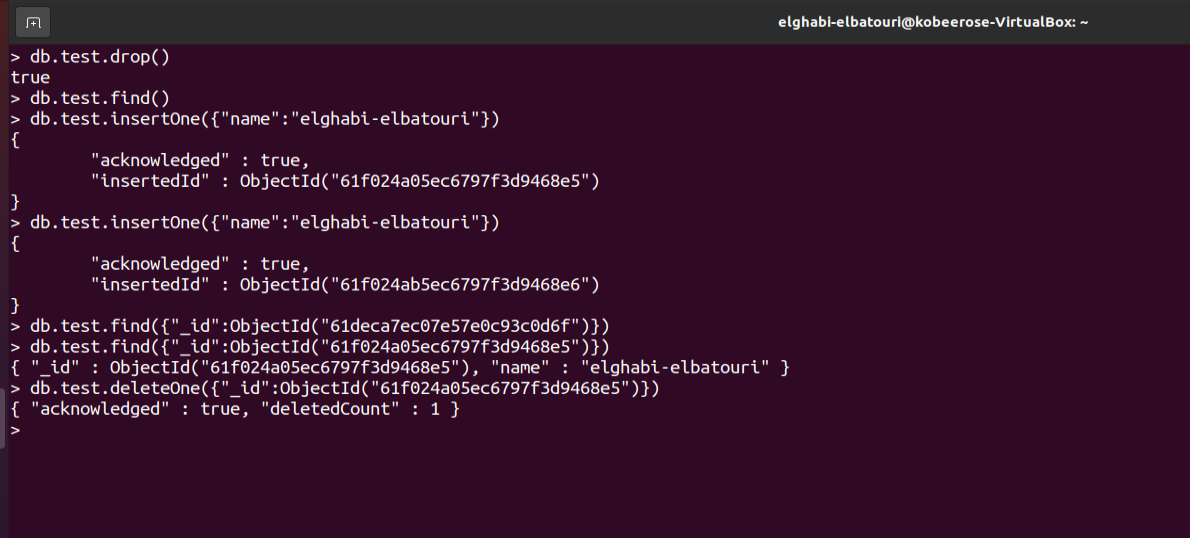
\includegraphics[width=1\linewidth]{Pictures/MongoDB/Examining MongoDB Query Features/Deleting and Updating documents/Delete documents} 
\end{center} 
\caption{Delete documents} 
\end{figure}  \FloatBarrier
\\

\par Lorem ipsum dolor sit amet, consectetur adipiscing elit. Aliquam facilisis massa quis orci volutpat, ut dictum tellus pulvinar. Nam vulputate diam a leo dignissim varius. Aenean nec tellus malesuada, tristique libero vitae, lacinia nibh. Donec quam libero, accumsan sollicitudin massa a, dictum gravida mauris
\\
\begin{figure}[!htb] 
\begin{center} 
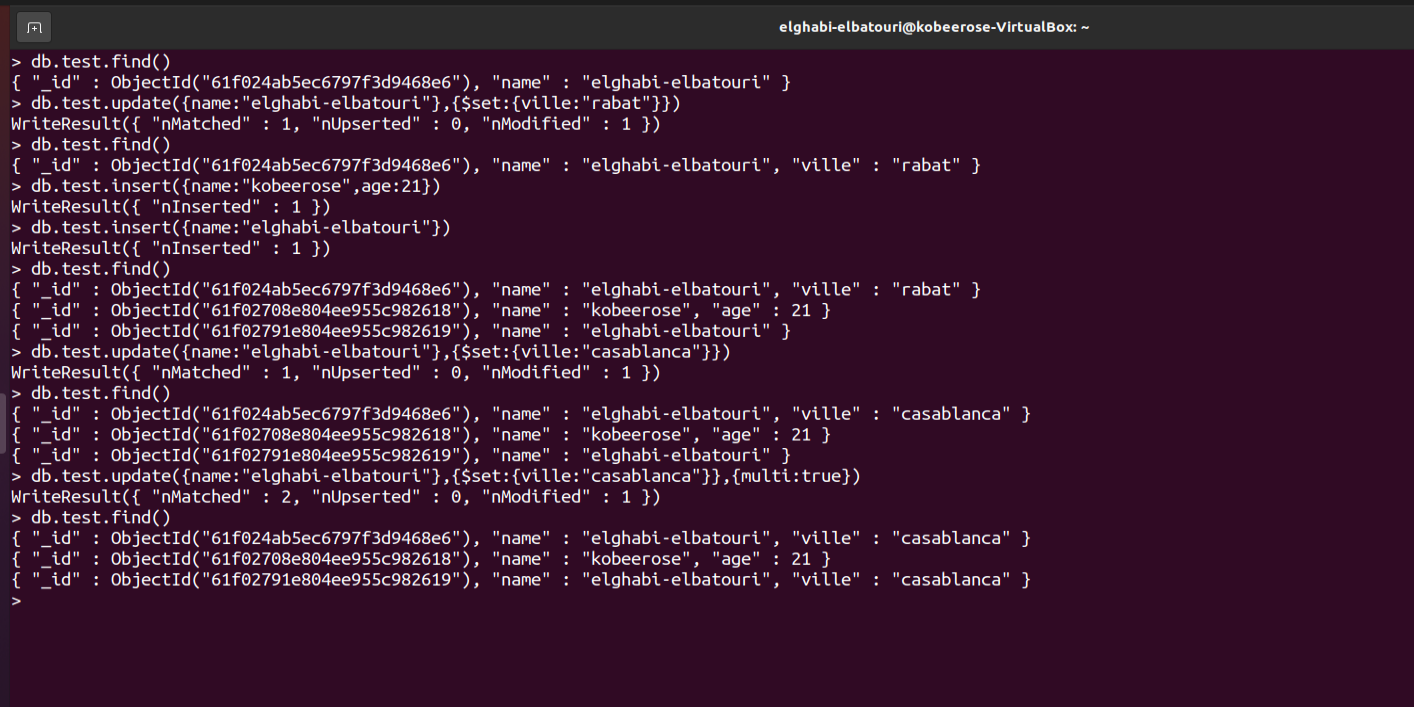
\includegraphics[width=1\linewidth]{Pictures/MongoDB/Examining MongoDB Query Features/Deleting and Updating documents/Updating documents} 
\end{center} 
\caption{Updating documents} 
\end{figure}  \FloatBarrier
\\

\par Lorem ipsum dolor sit amet, consectetur adipiscing elit. Aliquam facilisis massa quis orci volutpat, ut dictum tellus pulvinar. Nam vulputate diam a leo dignissim varius. Aenean nec tellus malesuada, tristique libero vitae, lacinia nibh. Donec quam libero, accumsan sollicitudin massa a, dictum gravida mauris
\\
\begin{figure}[!htb] 
\begin{center} 
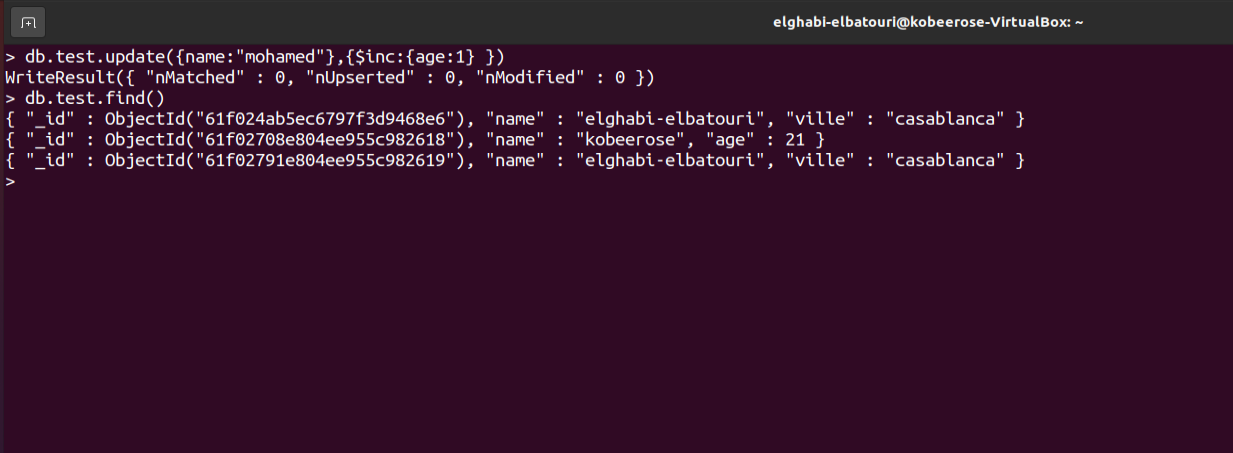
\includegraphics[width=1\linewidth]{Pictures/MongoDB/Examining MongoDB Query Features/Deleting and Updating documents/Increment a numeric field} 
\end{center} 
\caption{Increment a numeric field} 
\end{figure}  \FloatBarrier
\\

\par Lorem ipsum dolor sit amet, consectetur adipiscing elit. Aliquam facilisis massa quis orci volutpat, ut dictum tellus pulvinar. Nam vulputate diam a leo dignissim varius. Aenean nec tellus malesuada, tristique libero vitae, lacinia nibh. Donec quam libero, accumsan sollicitudin massa a, dictum gravida mauris
\\
\begin{figure}[!htb] 
\begin{center} 
\includegraphics[width=1\linewidth]{Pictures/MongoDB/Examining MongoDB Query Features/Deleting and Updating documents/Using \$push or \$pull operators} 
\end{center} 
\caption{Using \$push or \$pull operators} 
\end{figure}  \FloatBarrier

\end{spacing}